% !TEX root =  paper.tex

\section{Motivating Example}
\label{section:motivating-example}

\Cref{fig:motivating-example} illustrates a part of a sample UI mockup for a job hunting website.
The mockup, often designed by a graphics designer in a team, provides a visual representation of what the UI of the web app is supposed to look like.
The code corresponding to this mockup includes the \html code, which defines the mockup's structure and content, and \css code, which defines its style and presentation.
This code is typically generated automatically using popular web UI editors (e.g., Muse, Dreamweaver, Visual Studio).
The \html and \css code is interpreted by web browsers to render the UI.

Subsequently, a web developer oversees the creation of the final front-end code for the app.
For the vast majority of developers, a major part of this process is the creation of reusable components~\cite{StateOfJS:WebPlatformTests}.
Using components is key in improving modularity and maintainability and achieving the software engineering best practice of DRY (Don't Repeat Yourself).
It is also an effective way to remove duplications in the app's code,
which has been shown to be associated with 
increased error-proneness~\cite{Juergens:2009:DoCodeClonesMatter},
maintenance effort~\cite{Lozano:2008:AssessingTheEffectOfClones},
code instability~\cite{Mondal:2012:EmpiricalStudyCloneInstability}, 
as well as higher hosting costs and rendering delays due to the transmission of redundant data.
The utilization of reusable web components can help to address these issues.

For example, observe in \Cref{fig:motivating-example} that there are 
four groups of elements repeated in the mockup,
denoted by \circled{A}, \circled{B}, \circled{C} and \circled{D}.
Notice that the repeated elements are not exactly similar;
there are differences in terms of, for example, the text and images appearing within the elements.
Nevertheless, the structure of the repeated elements in each group and their overall visual appearances are unquestionably repeating. Reptitions in UI are unavoidable and neccessary. In fact, repetition is an important aspect of effective visual design~\cite{Meggs:1992:TypeAndImageGraphicDesign},
and is known as a \textit{functional technique} 
to achieve appealing designs~\cite{Dondis:1974:VisualLiteracy}.
Research has shown that, when a \textit{visual stimuli} is repeated,
it is more likely to be accepted by people,
a phenomenon called \textit{repeated exposure}~\cite{William:2010:UniversalPrinciplesOfDesign}.

\begin{figure}
    \centering
    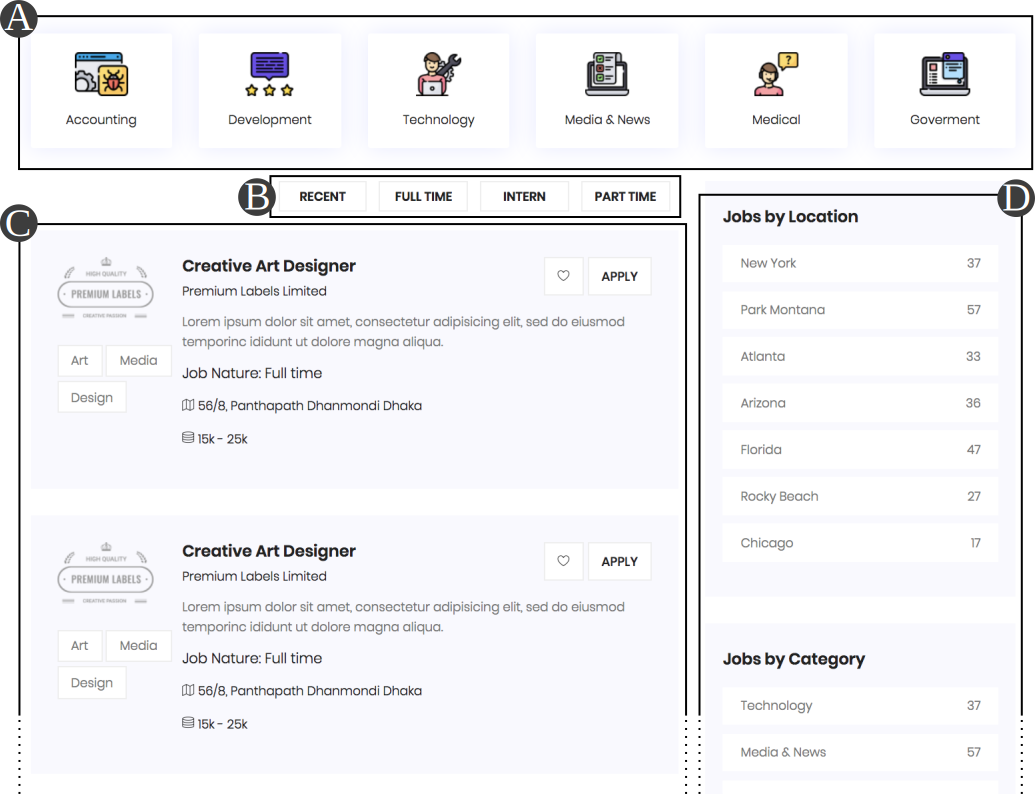
\includegraphics[width=0.8\textwidth]{maintainability/figures/motivating-example}
    \caption{An example of a web UI mockup.}
    \label{fig:motivating-example}
\end{figure} 


However, the process of creating reusable components is rather time consuming, 
requiring manual effort~\cite{thinking:in:components}.
When analyzing repetitions in a mockup
to construct components in one of the modern UI frameworks,
developers often face the following challenges:
\begin{itemize}[leftmargin=*]
	\item They need to visually glance at the mockup and manually identify the patterns in the UI
	that can be potentially refactored to create a reusable component.
	For instance, for group \circled{A}, they need to find all patterns in 
	the page that represents components similar to the elements inside
	group \circled{A}.
	The repetition might be spread across the web page,
	making the identification more challenging.
	The developer has to repeat this same process for other groups of components on the page, which quickly becomes a time consuming manual effort. 
	Note that, this identification is not possible by only using existing code clone detection tools
	that support \html code as input (e.g., \nicad~\cite{Roy:2008:NiCad}),
	due to several reasons:
	
	\begin{enumerate}[leftmargin=*]
		\item These tools leave out the visual appearance of the elements 
	and only work at the source code level, which is sub-optimal since there are several \textit{inherent patterns}
	in \html which do not necessarily represent a UI component. 
	For example, \html tables are declared using a \code{<table>} tag
	followed by a series of other tags, e.g., 
	\code{<thead>}, \code{<tbody>}, 
	\code{<colgroup>},
	\code{<tr>}, and \code{<td>},
	nested in a predefined hierarchy.
	The clone detector might mark all tables on the page for extraction, even if they do not visually constitute a reusable component in the UI.
	The same happens for several other elements, such as (un)ordered, description, and drop-down lists.	

	\item Clone detectors need to be configured properly in order to yield desirable clones.
	There is usually a large list of parameters and thresholds to tune,
	and finding an optimal configuration is a laborious task~\cite{Wang:2013:SearchingForBetterConfigs}.
	
	\item Clone detectors are not aware of the ultimate reason for detecting clones,
	e.g., there is no configuration that can force them to only identify clones that can be unified into a component template. 

	\end{enumerate}
		
	\item The developer also needs to \textit{unify} the patterns
	to construct a reusable component in a UI framework.
	This process needs careful investigation of repeated \html,
	to identify how elements can be unified into one representative component,
	and which elements can be \textit{parameterized} when there are differences.
	For example, in group \circled{A}, a developer would examine each button in the group, and determine which parts are repeated between the buttons, and which part is variable (e.g., the button icon and its label).
	The constructed component should resemble the exact hierarchy of the original repeated elements,
	or else the output of the resulting UI might differ from the original one.
	
	 
	\item Moreover, to use the constructed component,
	the developer has to \textit{instantiate} it
	in the places where the repeated elements originally appeared,
	with the appropriate parameters (e.g., original texts or images)
	to preserve the output of the mockup.
	For example, in group \circled{A}, the developer needs to refactor the original code and replace every occurrence of a button with a call to the button component, passing along arguments for the button label and its image.
\end{itemize}

To the best of our knowledge, there has been no techniques 
available to address the aforementioned issues and 
support developers in the generation of components.






